% Chapter Template

% Main chapter title
%\chapter[toc version]{doc version}
\chapter{Multi-source domain adaptation}

% Short version of the title for the header
%\chaptermark{version for header}

% Chapter Label
% For referencing this chapter elsewhere, use \ref{ChapterTemplate}
\label{chp:domain_adaptation}

% Write text in here
% Use \subsection and \subsubsection to organize text

\begin{tcolorbox}
	\small{
		Some parts of this chapter were originally published in or adapted from:
		\begin{itemize}
			\item[] \cite{ThesisFrancisco} \bibentry{ThesisFrancisco} (presented in \Secref{sec:da_sensors})
			\item[] \cite{MODAFM} \bibentry{MODAFM} (presented in \Secref{sec:modafm})
		\end{itemize}
		
		The Master's thesis \cite{ThesisFrancisco} was supervised by Jaime S. Cardoso and co-supervised by Diogo Pernes.
	}
\end{tcolorbox}

\section{Introduction}
\label{sec:chp3_intro}
In Chapter \ref{chp:networked_data_streams}, we have addressed the situation where the set of entities was the same at training and testing time. The goal there was to exploit inter-correlations between entities to learn better generative models for each individual entity. Now, we focus on the problem of learning a discriminative model for one particular entity (the \newterm{target}) for which no annotated data is available. Assuming some invariance properties, we can hope to accomplish this task by learning a discriminative model using the combination of annotated data from the remaining entities (the \newterm{sources}) and unlabeled data from the target entity. Since entities do not need to (and generally do not) correspond to physical objects and may refer to different contexts where the data was collected, they are more commonly called \newterm{domains} and the problem itself is known as \newterm{domain adaptation} (DA). In the following, we motivate the practical importance of this problem and summarize our contributions.

Supervised training of deep neural networks has achieved outstanding results on multiple learning tasks greatly due to the availability of large and rich annotated datasets. Unfortunately, annotating such large-scale datasets is often prohibitively time-consuming and expensive. Furthermore, in many practical cases, it is not possible to collect annotated data with the same characteristics as the test data, and, as a result, training and test data are drawn from distinct underlying distributions. As a consequence, the model performance tends to decrease significantly on the test data. The goal of DA algorithms is to minimize this gap by finding transferable knowledge from the source to the target domain. Sometimes, it is assumed that a small portion of labeled target data are available at training time -- a setting that is known as \newterm{semi-supervised} DA (e.g.\ \citet{Daume2010, Donahue2013, Kumar2010, Saito2019, Yao2015}). In this chapter, we focus mostly on the more challenging scenario, where no labeled target data are available for training -- known as \newterm{unsupervised} DA (e.g.\ \citet{Baktashmotlagh2013, Ganin2015, Kang2019, Long2016, Zhao2018}). The DA problem, in its semi-supervised and unsupervised variants, has received increased attention in recent years, both from theoretical (e.g.\ \citet{BenDavid2010, BenDavid2007, Blitzer2008, Cortes2014, Gopalan2013, Hoffman2018, Zhao2019}) and algorithmic perspectives (e.g.\ \citet{Ajakan2014, Becker2013, Fernando2013, Jhuo2012, Long2015, Louizos2015, Sun2016, Tzeng2017}). In many situations, the annotated training data may consist of a combination of distinct datasets, some of which may be closer or further away from the target data. Finding nontrivial ways of combining multiple datasets to approximate the target distribution and extracting relevant knowledge from such combination is the purpose of multi-source DA algorithms (e.g.\ \citet{Kim2017, Guo2018, Hoffman2018, Mansour2009, Sebag2019, Zhang2015, Zhao2018}) and is also our main focus in this chapter.

The remainder of the chapter is organized as follows: i) we formalize the problem and provide some useful background by reviewing some important theoretical results and state of the art algorithms (\Secref{sec:chp3_background}); ii) we discuss some exploratory solutions for this problem in the context of sensor networks (\Secref{sec:da_sensors}); and finally iii) we present our own novel algorithm for multi-source domain adaptation (\Secref{sec:modafm}).

\section{Background}
\label{sec:chp3_background}
We start by analyzing the problem of DA from a theoretical perspective and then we overview the main approaches that constitute the state of the art. Although some authors have considered the problem of DA for regression problems (e.g.\ \cite{Cortes2011}, \cite{Zhao2018}), the literature on classification is far more vast. Moreover, many of the results and methods explained in this section can be extended to regression problems with minor modifications. For these reasons, we shall focus our discussion mostly on classification.

\subsection{Theoretical foundation}
\label{sec:da_theory}

\subsubsection{Single source setting}
\label{sec:da_theory_ss}
\citet{BenDavid2010} developed a rigorous yet comprehensive theoretical model for domain adaptation that we summarize here. This formulation enlightens the intrinsic difficulties associated with this task and provides a deep foundation for many of the algorithms we discuss in this chapter and, particularly, to our own approach, presented in \Secref{sec:modafm}.

Before we present and discuss the most important results, let us introduce a few preliminary definitions. A \newterm{domain} $\gD$ is defined by a joint distribution $p_\gD(\rvx, \rvy)$ over input features $\rvx \in \gX$ and target variables $\rvy \in \gY$, where $\gX$ and $\gY$ denote the input and target spaces, respectively. For the domain adaptation task to be well defined, at least two domains must be considered: a \newterm{source} domain $\gS$, with joint distribution denoted by $p_\gS(\rvx, \rvy)$, from which abundant annotated data is usually available, and a \newterm{target} domain $\gT$, with joint distribution $p_\gT(\rvx, \rvy)$, from which scarce or even zero annotated data is available at training time. Following most classical results from statistical learning theory, \citet{BenDavid2010} focused on binary classification, thus $\gY = \{0, 1\}$. Under this setting, it is possible to define a \newterm{labeling function} $f_\gD: \gX \mapsto [0, 1]$ for each domain, given by $f_\gD(\vx) = p_\gD(\ry=1 \mid \vx)$. A \newterm{hypothesis} is any function $h: \gX \mapsto \{0,1\}$ and a set $\gH$ of these functions is called a \newterm{hypothesis class}. The expected absolute difference between $h$ and $f_\gD$ is called the \newterm{risk} (or \newterm{error}) of hypothesis $h$ (with respect to the labeling function $f_\gD$):
\begin{equation}
	\label{eq:risk}
	\epsilon(h,f_\gD) \triangleq \E_{\rvx \sim p_\gD} |h(\rvx) - f_\gD(\rvx)|.
\end{equation}
We use $\epsilon_\gS(h)$ and $\epsilon_\gT(h)$ as shorthands for $\epsilon(h,f_\gS)$ and $\epsilon(h,f_\gT)$ and refer to them as the source and target risks (or errors), respectively. The empirical estimates of these are denoted as $\widehat{\epsilon}_\gS(h)$ and $\widehat{\epsilon}_\gT(h)$, respectively.

Given two domains $\gD$ and $\gD'$ and a hypothesis class $\gH$, the $\gH$-divergence provides a distance measure between the marginal distributions of features in $\gD$ and $\gD'$ (according to $\gH$):
\begin{equation*}
	\label{eq:h_div}
	d_{\gH}(\gD,\gD') \triangleq \sup_{h \in \gH} 2 |\mathrm{Pr}_{\gD}(\1_h) - \mathrm{Pr}_{\gD'}(\1_h)|,
\end{equation*}
where $\1_h \triangleq \{\vx \in \gX: h(\vx)=1\}$ and $\mathrm{Pr}_{\gD}(\1_h)$ is the probability assigned by the distribution $p_\gD(\rvx)$ to the subset $\1_h \subseteq \gX$. As is often the case, when the true underlying marginal distributions are unknown or intractable but finite sets of (unlabeled) samples from both domains are available, an empirical $\gH$-divergence can be constructed by replacing the true probabilities $\mathrm{Pr}_{\gD}(\1_h)$ and $\mathrm{Pr}_{\gD'}(\1_h)$ by the respective empirical estimates. Remarkably, under weak conditions on the hypothesis class, computing this empirical $\gH$-divergence is equivalent to finding the hypothesis in $\gH$ that maximally discriminates between samples of the two domains. This result is enunciated formally in Lemma \ref{lemma:emp_h_div} and, as we shall see later, is exploited by adversarial-based approaches for domain adaptation.
\begin{lemma}
	\label{lemma:emp_h_div}
	(Lemma 2 from \citet{BenDavid2010}) Let $\gH$ be a hypothesis class such that if $h \in \gH$ then $1-h \in \gH$. Given two sets $\widehat{D}$ and $\widehat{D}'$ of $n$ samples each drawn from two domains $D$ and $D'$, the empirical $\gH$-divergence between $D$ and $D'$ is given by:
	\begin{equation}
		\widehat{d}_{\gH}(\gD,\gD') = 2 \left(1 - \min_{h \in \gH} \left[\frac{1}{n} \sum_{\vx: h(\vx)=1} \1_{\vx \in \widehat{\gD}} + \frac{1}{n} \sum_{\vx: h(\vx)=0} \1_{\vx \in \widehat{\gD}'}\right]\right).
	\end{equation}
\end{lemma}
Note that if the two sets $\widehat{\gD}$ and $\widehat{\gD}'$ can be discriminated perfectly by a hypothesis $h \in \gH$ (i.e.\ if there is an $h \in \gH$ such that $h(\vx) = 0$ if $x \in \widehat{\gD}$ and $h(\vx) = 1$ if $x \in \widehat{\gD}'$), then $\widehat{d}_{\gH}(\gD,\gD')$ is maximum and equal to 2.

For a hypothesis class $\gH$, we may define the \newterm{symmetric difference hypothesis class} $\gH \Delta \gH$ as:
\begin{equation}
\label{eq:h_delta_h}
\gH \Delta \gH \triangleq \{l: l(\vx) = h(\vx) \oplus h'(\vx), \; h, h' \in \gH\},
\end{equation}
where $\oplus$ denotes the ``exclusive or" (xor) operation. Combining this definition with \eqref{eq:h_div}, the definition of $\gH \Delta \gH$-divergence, which happens to play a major role in Theorem \ref{thm:da_bound_single_source}, follows immediately. This theorem is the main result in this section as it provides an upper bound for the target risk given the source risk and the $\gH \Delta \gH$-divergence between the source and target domains.
\begin{theorem}
	\label{thm:da_bound_single_source} (Theorem 2 from \citet{BenDavid2010}) Let $\gH$ be a hypothesis class with VC-dimension $d$. Consider $n$ unlabeled samples drawn from each of the two domains $\gS$ (source) and $\gT$ (target). Then, for every $h \in \gH$ and any $\delta \in (0,1)$, with probability at least $1-\delta$ over the choice of samples,
	\begin{equation}
		\label{eq:da_bound_single_source}
		\epsilon_\gT(h) \leq \epsilon_\gS(h) + \frac{1}{2} \widehat{d}_{\gH \Delta \gH}(\gS, \gT) + \lambda + 2\sqrt{\frac{2d\log(2n) + \log(\frac{2}{\delta})}{n}},
	\end{equation}
	where $\lambda \triangleq \min_{h \in \gH} \epsilon_\gS(h) + \epsilon_\gT(h)$.
\end{theorem}
This bound immediately confirms the intuition that a low target error can be achieved by training a classifier to minimize the error in the source domain, provided that the marginal distributions of features are similar (i.e.\ $\widehat{d}_{\gH \Delta \gH}(\gS, \gT)$ is small) and a low error on the combination of the two domains can be achieved (i.e.\ $\lambda$ is also small). A deeper and more complete interpretation of this bound shall be provided later on, when we take into account the fact that, by applying deep neural networks, we can not only construct rich hypothesis classes but also manipulate and learn feature representations. The latter observation suggests that this kind of the classifiers may also have an impact on the $\widehat{d}_{\gH \Delta \gH}(\gS, \gT)$ and $\lambda$ terms in \eqref{eq:da_bound_single_source}, which will indeed be the case.

\subsubsection{Multi-source setting}
\label{sec:da_theory_ms}
So far we have only considered the setting where a single source domain was available. However, in many practical cases, the annotated training dataset consists of a collection of subdatasets, each one belonging to its own domain. Therefore, it makes sense to consider $k$ distinct source domains $\gS_1, \gS_2, \dots, \gS_k$ and, in particular, to see how Theorem \ref{thm:da_bound_single_source} can be generalized to this setting.
\begin{theorem}
	\label{thm:da_bound_multi_source}
	(Theorem 2 from \citet{Zhao2018}) Let $\gH$ be a hypothesis class with VC-dimension $d$. Consider $n$ unlabeled samples drawn from the target domain $\gT$ and $n/k$ annotated samples drawn from each of the $k$ source domains $\gS_1, \gS_2, \dots, \gS_k$. Then, for every $h \in \gH$, any $\valpha \in [0,1]^k: \sum_{j=1}^k \evalpha_i = 1$, and any $\delta \in (0,1)$, with probability at least $1-\delta$ over the choice of samples,
	\begin{equation}
		\label{eq:da_bound_multi_source}
		\epsilon_\gT(h) \leq \sum_{j=1}^k \evalpha_j \left(\widehat{\epsilon}_{\gS_j}(h) + \frac{1}{2} \widehat{d}_{\gH \Delta \gH}(\gS_j, \gT)\right) + \lambda_\valpha + O \left(\sqrt{\frac{1}{n} \left(\log \frac{1}{\delta} +d \log \frac{n}{d} \right)} \right),
	\end{equation}
	where $\lambda_\valpha \triangleq \min_{h \in \gH} \epsilon_\gT(h) + \sum_{j=1}^k \evalpha_j \epsilon_{\gS_j}(h)$.
\end{theorem}
Unsurprisingly, the bound in Theorem \ref{thm:da_bound_multi_source} is essentially a convex combination of the bounds provided by Theorem \ref{thm:da_bound_single_source} for each individual source domain. Thus, the same interpretation applies here. Nonetheless, the source weights $\valpha$ provide an extra degree of freedom that should be taken into account. Depending on how much each source domain differs from the target, it may be beneficial to weight each source domain differently. Adjusting these weights is therefore an extra non-trivial task, exclusive to the multi-source setting, that may have a significant impact in the performance of the domain adaptation algorithm.

\subsection{State of the art}
\label{sec:da_sota}
We now do a brief overview of the most relevant DA algorithms, both in the single source and multi-source settings. 

As we have just seen from a theoretical point of view, the success of the DA task depends on how similar the target domain is to the source(s), which is equivalent to saying that some properties of the underlying distributions must be invariant across domains. Different DA algorithms can therefore be categorized according to the invariance properties they assume.

\subsubsection{Target shift}
\label{sec:target_shift_sota}
\begin{figure}
	\centering
	\begin{tikzpicture}[every loop/.style={},thick,
		main node/.style={circle,draw},font=\sffamily\Large\bfseries]
		
		\node[main node,minimum size=1.5cm] (D) {$\gD$};
		\node[main node,minimum size=1.5cm] (y) [right=1.5cm of D] {$\ry$};
		\node[main node,minimum size=1.5cm] (x) [right=1.5cm of y] {$\rvx$};
		
		\draw[->]
		(D) edge (y)
		(y) edge (x);
		
	\end{tikzpicture}
	\caption{Graphical representation of the target shift setting as a Bayesian network.}
	\label{fig:target_shift}
\end{figure}
In the \newterm{target shift} setting, only the marginal distribution of labels is allowed to vary across domains. A practical example where this assumption may be realistic is when the label $\ry$ represents having or not a certain disease and the input features $\rvx$ are symptoms. It is plausible to assume that the prevalence of the disease may vary over time or across different populations, but the probability of some symptom being present or absent given that one has or not the disease should remain constant. Thus, as represented in \Figref{fig:target_shift}, the joint distribution of any domain $\gD$ is assumed to factorize as $p_\gD(\rvx, \ry) = p(\rvx \mid \ry) p_\gD(\ry)$, where $p(\rvx \mid \ry)$ is domain-invariant. By further assuming that $\mathrm{Supp}(p_\gT(\ry)) \subseteq \mathrm{Supp}(p_\gS(\ry))$, we have:
\begin{align}
	p_\gT(\ry \mid \rvx) &\propto p(\rvx \mid \ry) p_\gT(\ry) \nonumber\\
	&= p(\rvx \mid \ry) p_\gS(\ry) \frac{p_\gT(\ry)}{p_\gS(\ry)} \nonumber\\
	&\propto p_\gS(\ry \mid \rvx) \frac{p_\gT(\ry)}{p_\gS(\ry)}.
\end{align}
Thus, if the class ratios $p_\gT(\ry)/p_\gS(\ry)$ are known, the problem of DA under target shift is solved by learning a probabilistic classifier on the source domain, reweighting it with the class ratios, and then normalizing the class scores. Therefore, the literature for DA under target shift focuses on estimating class ratios when these are unknown and cannot be estimated directly from the training data, due to the absence of labels for the target samples.

An elegant and simple solution for this problem was proposed by \citet{Lipton2018}. Specifically, for any classifier $h: \gX \mapsto \gY$ trained with labeled data from the source domain, the target shift assumption implies that $p_{\gT}(h(\rvx) \mid \ry) = p_{\gS}(h(\rvx) \mid \ry)$ and hence:
\begin{align}
p_{\gT}(h(\rvx)) &= \sum_{\ry} p_{\gT}(h(\rvx) \mid \ry) p_{\gT}(\ry) \nonumber\\
\allowdisplaybreaks
&= \sum_{\ry} p_{\gS}(h(\rvx) \mid \ry) p_{\gT}(\ry) \label{eq:estim_class_dist}\\
\allowdisplaybreaks
&= \sum_{\ry} p_{\gS}(h(\rvx), \ry) \frac{p_{\gT}(\ry)}{p_{\gS}(\ry)}. \label{eq:estim_class_ratio}
\end{align}
Note that $p_{\gS}(h(\rvx) \mid \ry)$, $p_{\gS}(h(\rvx), \ry)$, and $p_{\gS}(\ry)$ can all be estimated from labeled source samples and $p_{\gT}(h(\rvx))$ can be estimated from unlabeled target samples. Thus, one can either use \eqref{eq:estim_class_dist} to estimate $p_{\gT}(\ry)$ or \eqref{eq:estim_class_ratio} to estimate class ratios directly.

Other approaches involve learning class-dependent weights to match the mean conditional features of source data with the mean marginal features of target data in a reproducing kernel Hilbert space (e.g.\  \citet{Iyer2004}, \citet{Zhang2013}), or require density estimation to model $p(\rvx \mid \ry)$ (e.g.\ \citet{Chan2005}, \citet{Storkey2009}).

\subsubsection{Conditional shift}
\label{sec:cond_shift_sota}
\begin{figure}
	\centering
	\begin{tikzpicture}[every loop/.style={},thick,
	main node/.style={circle,draw},font=\sffamily\Large\bfseries]
	
	\node[main node,minimum size=1.5cm] (y) {$\ry$};
	\node[main node,minimum size=1.5cm] (x) [right=1.5cm of y] {$\rvx$};
	\node[main node,minimum size=1.5cm] (D) [right=1.5cm of x] {$\gD$};
	
	\draw[->]
	(y) edge (x)
	(D) edge (x);
	
	\end{tikzpicture}
	\caption{Graphical representation of the conditional shift setting as a Bayesian network.}
	\label{fig:cond_shift}
\end{figure}
In the \newterm{conditional shift} setting, the marginal distribution of labels is constant and the conditional of features given labels may change across domains. This scenario is represented in \Figref{fig:cond_shift}, from which it becomes clear that the joint distribution takes the form $p_{\gD}(\rvx, \ry) = p(\ry) p_{\gD}(\rvx \mid \ry)$, where $p(\ry)$ is domain-invariant. Besides being less realistic than other assumptions, DA under conditional shift is in general an ill-posed problem. Nonetheless, \citet{Zhang2013} show that identifiability of $p_{\gT}(\rvx \mid \ry)$ holds when it is assumed that, for any given $y$, $p_{\gT}(\rvx \mid y)$ only differs from $p_{\gS}(\rvx \mid y)$ in location and scale and derive a kernel-based approach to estimate these parameters.

\subsubsection{Concept shift}
\label{sec:concept_shift_sota}
\begin{figure}
	\centering
	\begin{tikzpicture}[every loop/.style={},thick,
	main node/.style={circle,draw},font=\sffamily\Large\bfseries]
	
	\node[main node,minimum size=1.5cm] (x) {$\rvx$};
	\node[main node,minimum size=1.5cm] (y) [right=1.5cm of x] {$\ry$};
	\node[main node,minimum size=1.5cm] (D) [right=1.5cm of y] {$\gD$};
	
	\draw[->]
	(x) edge (y)
	(D) edge (y);
	
	\end{tikzpicture}
	\caption{Graphical representation of the concept shift setting as a Bayesian network.}
	\label{fig:concept_shift}
\end{figure}
\newterm{Concept shift} refers to the situation where the marginal feature distributions $p(\rvx)$ are constant but the conditional distribution of the target variable $p_{\gD}(\ry \mid \rvx)$ is domain-dependent, thus $p_{\gD}(\rvx, \ry) = p(\rvx)p_{\gD}(\ry \mid \rvx)$, as implied by \Figref{fig:concept_shift}. When the change happens over time, this setting is also known as \newterm{concept drift} (\citet{Webb2018}). The literature on concept drift is vast and focuses mostly on the detection of its occurrence so that the model can be updated using new data. \citet{Gama2014} overview the most popular techniques to address this problem.

\subsubsection{Covariate shift}
\label{sec:cov_shift_sota}
\begin{figure}
	\centering
	\begin{tikzpicture}[every loop/.style={},thick,
	main node/.style={circle,draw},font=\sffamily\Large\bfseries]
	
	\node[main node,minimum size=1.5cm] (D) {$\gD$};
	\node[main node,minimum size=1.5cm] (x) [right=1.5cm of D] {$\rvx$};
	\node[main node,minimum size=1.5cm] (y) [right=1.5cm of x] {$\ry$};
	
	\draw[->]
	(D) edge (x)
	(x) edge (y);
	
	\end{tikzpicture}
	\caption{Graphical representation of the covariate shift setting as a Bayesian network.}
	\label{fig:cov_shift}
\end{figure}
\newterm{Covariate shift} is by far the most common assumption and therefore the most widely addressed setting in the DA literature. As implied by the graphical representation in \Figref{fig:cov_shift}, here the conditional distribution of labels given features is constant and the marginal distribution of features is domain-dependent. Thus, $p_\gD(\rvx, \ry) = p(\ry \mid \rvx) p_\gD(\rvx)$, where $p(\ry \mid \rvx)$ is constant across domains. This assumption might hold for instance in image classification problems where the domain shift is caused by different sensors or lighting conditions.

Since $p_\gT(\ry \mid \rvx) = p_\gS(\ry \mid \rvx)$, infinite labeled data from the source domain and a consistent estimator of this conditional distribution would solve this DA task. However, the former is obviously unrealistic and therefore the problem should be analyzed taking into account that the available data is finite. Let $\ell(\cdot, \cdot)$ be any loss function for the supervised learning problem. The goal is then to find an unbiased estimator of the target loss $\E_{\rvx, \ry \sim p_\gT} \ell(h(\rvx),\ry)$ when no labeled samples from the target domain are available. Following \citet{Sugiyama2007}, if the marginal densities $p_\gS(\rvx)$ and $p_\gT(\rvx)$ are known and assuming $\mathrm{Supp}(p_\gT(\rvx)) \subseteq \mathrm{Supp}(p_\gS(\rvx))$, this estimator can be obtained using \newterm{importance weights} $w(\rvx) \triangleq p_\gT(\rvx)/p_\gS(\rvx)$:
\begin{align}
	\E_{\rvx, \ry \sim p_\gT} \ell(h(\rvx),\ry) &= \sum_{\ry} \int l(h(\rvx),\ry) p_\gT(\rvx, \ry) d\rvx \nonumber\\
	&= \sum_{\ry} \int \ell(h(\rvx),\ry) p(\ry \mid \rvx) p_\gT(\rvx) d\rvx \nonumber\\
	&= \sum_{\ry} \int \frac{p_\gT(\rvx)}{p_\gS(\rvx)} \ell(h(\rvx),\ry)  p(\ry \mid \rvx) p_\gS(\rvx) d\rvx \nonumber\\
	&= \sum_{\ry} \int w(\rvx) \ell(h(\rvx),\ry)  p_\gS(\rvx, \ry) d\rvx \nonumber\\
	&= \E_{\rvx, \ry \sim p_\gS} w(\rvx) \ell(h(\rvx),\ry).
\end{align}
Hence, $(1/n) \sum_{i=1}^{n} w(\vx_i) \ell(h(\vx_i),y_i)$ is an unbiased estimator of the target loss, constructed using only source data, which can therefore be used as the loss for the supervised learning problem. When the marginal distributions are unknown and the feature space is low-dimensional, kernel density estimation techniques can be employed to estimate them (e.g.\ \citet{Shimodaira2000,Sugiyama2007,Cortes2010}). An alternative that removes the constraint on the support of the marginal target distribution is learning a transformation $T: \gX \mapsto \gX$ such that $p_{\gS}(T(\rvx)) = p_{\gT}(\rvx)$, which can be accomplished using optimal transport theory (\citet{Courty2015}). Later approaches aim to relax the covariate shift assumption by trying to align the joint source and target distributions (\citet{Courty2017}) and extend the same principles to the multi-source setting (\citet{Turrisi2020}).

For high-dimensional data (e.g.\ images), where the marginal distributions are typically unknown and hard to estimate from finite data, deep learning models play an important role by providing a successful tool learn semantically rich low-dimensional feature representations. It is then possible to learn a function $g:\gX \mapsto \gZ$ mapping input data to a new feature space $\gZ$ such that $p_{\gT}(g(\rvx))/p_{\gS}(g(\rvx)) \approx 1$, i.e.\ where the marginal feature distributions of the two domains coincide. This approach has the additional benefit of moving the overlapping support assumption to a lower-dimensional space, where it is less likely to be violated than in the original space (e.g.\ pixel space). In this new feature space the covariate shift has vanished and therefore any classifier $h:\gZ \mapsto \gY$ that achieves low error on the source domain will also perform well in the target. An alternative way of motivating these approaches follows from analyzing again the target risk bound provided in \eqref{eq:da_bound_single_source}. When we presented this bound, we assumed for simplicity that the feature space was fixed and therefore the upper bound would be minimized by minimizing the source risk. However, if the feature space can itself be optimized, the term $\widehat{d}_{\gH \Delta \gH}(\gS, \gT)$ can be minimized by finding a feature space where the source and target marginal distributions coincide. This idea has been exploited extensively in recent years, either by matching the distributions using maximum mean discrepancy (e.g.\ \citet{Long2015,Guo2018}) or, in most cases, using an adversarial neural network (e.g.\ \citet{Zhao2018,Ganin2015,Pei2018,Sebag2019}).

Adversarial-based DA was originally introduced by \citet{Ganin2015} and results from the observation that 
computing $\widehat{d}_{\gH \Delta \gH}(\gS, \gT)$ is equivalent to finding a classifier that maximally discriminates between samples of the source and target domains (Lemma \ref{lemma:emp_h_div}). Intuitively, if no classifier exists that can distinguish between source and target features, then the distributions of these two must coincide. Thus, if we have access to sets $\widehat{\gS}$ and $\widehat{\gT}$ of labeled samples from the source domain and unlabeled samples from the target, respectively, we can train a feature extractor network $g:\gX \mapsto \gZ$, a classifier $h:\gZ \mapsto \gY$, and a domain discriminator $d:\gZ \mapsto \{0,1\}$ to solve the following minimax problem\footnote{This objective is merely formal since the 0-1 loss is non-smooth and intractable. In practice, the usual classification losses are used instead.}:
\begin{equation}
	\label{eq:dann_obj}
	\min_{g,h} \max_d \quad \widehat{\epsilon}_\gS(h \circ g) + 1 - \left(\frac{1}{n} \sum_{\vx: d(g(\vx))=1} \1_{\vx \in \widehat{\gS}} + \frac{1}{n} \sum_{\vx: d(g(\vx))=0} \1_{\vx \in \widehat{\gT}}\right),
\end{equation}
where $\circ$ denotes function composition. Several variations to this idea have been proposed so far, aiming to extend it to the multi-source setting (\citet{Zhao2018}), or beyond the covariate shift assumption (\citet{Pei2018}), or both (\citet{Sebag2019}).

\subsubsection{Invariance of causal mechanisms}
\label{sec:causal_da_sota}
The settings we have discussed so far consider all features $\rvx$ as atomic and hence do not take into account how different features interact to produce the target variable $\ry$.  Other approaches drop this limitation by decomposing the feature vector into individual features $\rx_1,\rx_2,\dots,\rx_m$, taking into account the structure of the causal Bayesian network governing the data generating process, and using causal inference tools to identify the target distribution. These methods assume that the flow of cause and effect cannot be reversed by domain shift and therefore changes in distribution are due to different interventions in the same causal graph $\gG$ (e.g.\ presence of additional exogenous variables inducing non-causal associations between features and the target variable). \citet{Bareinboim2016} assume $\gG$ is known and all interventions are perfect (i.e.\ all interventions consist of edge removal operations) and derive conditions for identifiability of $p_\gT(\ry \mid \cdots)$ given $\gG$ and $p_\gS(\rvx, \ry)$. \citet{Rojas2018} and \citet{Magliacane2018} relax the covariate shift setting by assuming that there exists a strict subset $\bar{\rvx} \subset \rvx$ such that $p_\gD(\ry \mid \bar{\rvx})$ is domain-invariant and propose algorithms to infer $\bar{\rvx}$ given data from multiple source domains.

Despite being (arguably) more trustworthy than purely data-driven approaches, cau-\allowbreak sality-based methods still struggle to be applied in practice. First of all, they depend to some extent on $\gG$ being given. In many applications, domain knowledge is insufficient to build such a graph. Moreover, causal discovery algorithms, which aim to learn the structure of the graph from data, are computationally expensive and, given observational data, can only recover $\gG$ up to its Markov equivalence class, at least when no parametric assumptions are made  (\citet{Peters2014}). Furthermore, these methods are unsuitable to be applied to image data as no meaningful causal reasoning can be built in pixel space and even deep neural networks are still incapable of finding suitable representations for this goal (\citet{Scholkopf2021}).

\section{Adversarial domain adaptation for object counting in videos}
\label{sec:da_sensors}

\subsection{Motivation}
As different sensors are added to and excluded from a network, we should take into account the fact that the sensors used at training time are different from the ones where the model will make predictions. Since domain shifts between different sensors on a sensor network are usually substantial, it is imperative that robust domain adaptation methods are developed that take into account the constraints of the sensor network.

There is a lack of domain adaptation methods focusing on how to handle the temporal component of data. \citet{Chen2019} proposed an algorithm called Temporal Attentive Alignment for implementing DA in video datasets that explicitly attends to temporal dynamics and \citet{Liu2014} proposed a spatio-temporal DA model named TrCbrBoost for classifying land use. It should be noted, though, that both of these works only deal with a single-source-single-target setting, which is simpler than the multi-source case present when dealing with sensor networks.

For dealing with a multi-source setting, adversarial approaches have proven successful. \citet{Zhao2018} introduced an algorithm called multi-source domain adversarial networks (MDAN) that makes use of $k$ domain discriminators that aim to distinguish between the target and the $k$ source domains. MDAN showed superior performance when compared to other state of the art methods on the task of counting vehicles in images obtained from city cameras videos. Given the positive results obtained, and given the fact that MDAN does not consider the temporal component of the video frames, we consider it is worthy to investigate the adaptation of this model so that it can receive a temporal sequence as an input.

The setting where sensors correspond to video cameras is especially interesting since video data is very high-dimensional. Moreover, the fact that different cameras are located in different places, and therefore have distinct points of view, increases the domain shift and therefore makes this task even more challenging.

Here, we shall explore how to adapt the MDAN model so that both of its adversarial networks are LSTM-based. We decided to go with this type of network since it has already shown promising results in our task: \citet{Zhang2017} introduced an LSTM network architecture for counting vehicles in images obtained from city cameras and reported an improvement of the mean absolute error when compared to other state of the art methods.

\subsection{MDAN: Multi-source domain adversarial networks}
\label{sec:da_sensors_mdan}
We now review the MDAN model introduced by \citet{Zhao2018}. This model is motivated by the target risk bound provided in Theorem \ref{thm:da_bound_multi_source} and is an extension to the multi-source setting of the single source model by \citet{Ganin2015}. Specifically, the following formal objective is considered:
\begin{equation}
	\min_{g,h} \max_{j \in \{1,\cdots,k\}} \quad \widehat{\epsilon}_{\gS_j}(h \circ g) + \frac{1}{2} \widehat{d}_{\gH \Delta \gH}(\gS^g_j, \gT^g),
\end{equation}
where $g: \gX \mapsto \gZ$ and $h: \gZ \mapsto \gY$ are, as before, the feature extractor and the classifier networks and $\gS^g_j$ and $\gT^g$ are, respectively, the $j$-th source domain and the target domain representations in the new feature space $\gZ$ (i.e.\ $p_{\gD^g}(\rvx) \triangleq p_\gD(g(\rvx))$ for any domain $\gD$). Here, the empirical $\gH \Delta \gH$-divergence between $\gS^g_j$ and $\gT^g$ is also implemented with an adversarial domain discriminator $d_j:\gZ \mapsto \{0,1\}$ aiming to discriminate between samples of the two domains. Thus, the model comprises $k$ domain discriminator networks, i.e.\ one for each source domain. This objective is therefore identical to \eqref{eq:dann_obj} with the only difference that, since here there are multiple source domains, the model is optimized for the hardest source domain at each training iteration. In this formulation, $\valpha$ in \eqref{eq:da_bound_multi_source} is a one-hot vector whose active component corresponds to the hardest source domain. Because the bound holds for any convex combination of source domains, the authors also explore a soft-max version of this problem, where smaller positive weights are assigned to the easier source domains:
\begin{equation}
\min_{g,h} \quad \frac{1}{\gamma} \log \sum_{j=1}^{k} \exp \left( \gamma( \widehat{\epsilon}_{\gS_j}(h \circ g) + \frac{1}{2} \widehat{d}_{\gH \Delta \gH}(\gS^g_j, \gT^g)) \right).
\end{equation}
Here, $\gamma > 0$ is a hyperparameter controlling the softness of the max operation ($\gamma \to \infty$ corresponds to the hard-max).

\subsubsection{The gradient reversal layer}
\label{sec:da_sensors_grad_rev}
Adversarial DA algorithms, of which MDAN is a particular case, all aim to solve some variant of the following minimax problem:
\begin{equation}
	\min_{\vtheta_g, \vtheta_h} \max_{\vtheta_d} \quad \left \lbrace L(\vtheta_g, \vtheta_h, \vtheta_d) =  L_{\text{task}}(\vtheta_g, \vtheta_h) - \lambda_d L_{\text{disc}}(\vtheta_g, \vtheta_d) \right \rbrace,
\end{equation}
where $L_{\text{task}}$ is the supervised loss for the desired task, $L_{\text{disc}}$ is the classification loss for the domain discrimination task, $\vtheta_g$, $\vtheta_h$, and $\vtheta_d$ are the parameters of the feature extractor, task executor, and domain discriminator networks, respectively, and $\lambda_d > 0$ is a hyperparameter. This is a treatable surrogate of objective \plaineqref{eq:dann_obj}.

Solving this problem then consists in finding a saddle point of this loss function. Using automatic differentiation libraries (e.g.\ PyTorch or TensorFlow), the naive solution would involve declaring two optimizers, one for the parameters $\vtheta_g$ and $\vtheta_h$ and another for $\vtheta_d$, and then performing gradient descent with the former and gradient ascent with the latter:
\begin{align}
	&\vtheta_g \leftarrow \vtheta_g - \rho \left(\nabla_{\vtheta_g}L_{\text{task}} - \lambda_d \nabla_{\vtheta_g} L_{\text{disc}}\right), \label{eq:grad_feature_extractor}\\
	&\vtheta_h \leftarrow \vtheta_h - \rho \nabla_{\vtheta_h}L_{\text{task}}, \label{eq:grad_task_executor}\\
	&\vtheta_d \leftarrow \vtheta_d + \rho \left(-\lambda_d \nabla_{\vtheta_d}L_{\text{disc}}\right), \label{eq:grad_discriminator}
\end{align}
where $\rho>0$ is the learning rate. This implies an extra computational burden because gradients need to be backpropagated through the discriminator network twice, one for computing $\nabla_{\vtheta_d} L_{\text{disc}}$ and another for computing $\nabla_{\vtheta_g} L_{\text{disc}}$.

The gradient reversal layer (\citet{Ganin2015}) is an ingenious solution for this problem. This layer is a pseudo-function $r$ that behaves as the identify in the forward pass but inverts the sign of the gradient in the backward, i.e.:
\begin{equation}
	r(\vx) \triangleq \vx, \quad \frac{\partial r}{\partial \vx} \triangleq -I.
\end{equation}
By placing it in between the feature extractor $g$ and the domain discriminator $d$, the gradient $\nabla_{\vtheta_g} L_{\text{disc}}$ will come with its sign inverted. Thus, performing gradient descent over all parameters of
\begin{equation}
	L_{\text{task}}(\vtheta_g, \vtheta_h) + \lambda_d L_{\text{disc}}(\vtheta_g, \vtheta_d),
\end{equation}
yields exactly update equations \plaineqref{eq:grad_feature_extractor}, \plaineqref{eq:grad_task_executor}, and \plaineqref{eq:grad_discriminator}.

\subsection{FCN-rLSTM: Spatio-temporal deep neural network for object counting}
\label{sec:da_sensors_fcn_rltsm}

\citet{Zhang2017} proposed FCN-rLSTM, a deep neural network architecture for counting vehicles in low-quality videos captured by city cameras that will constitute the backbone of our models. 

Although each video frame should contain all the information required to identify the number of vehicles in it, issues with the quality of the collected data can make vehicle counting a difficult problem, namely low resolution, vehicle occlusion, and different vehicle scales, particularly noticeable when the camera is too close to the road. Thus, assuming that the frame rate is sufficiently large when compared to the vehicles speed, leveraging information from the previous frames should help improving the accuracy of the prediction for the current frame. For this reason, FCN-rLSTM combines a fully convolutional network with a recurrent module, which preserves memory from the previous frames in LSTM cells. This is a density-based estimation method, being able to deal well with low frame rates, low resolutions, and vehicle occlusions, but having difficulty in accounting for different vehicle scales.

\begin{figure}
	\centering
	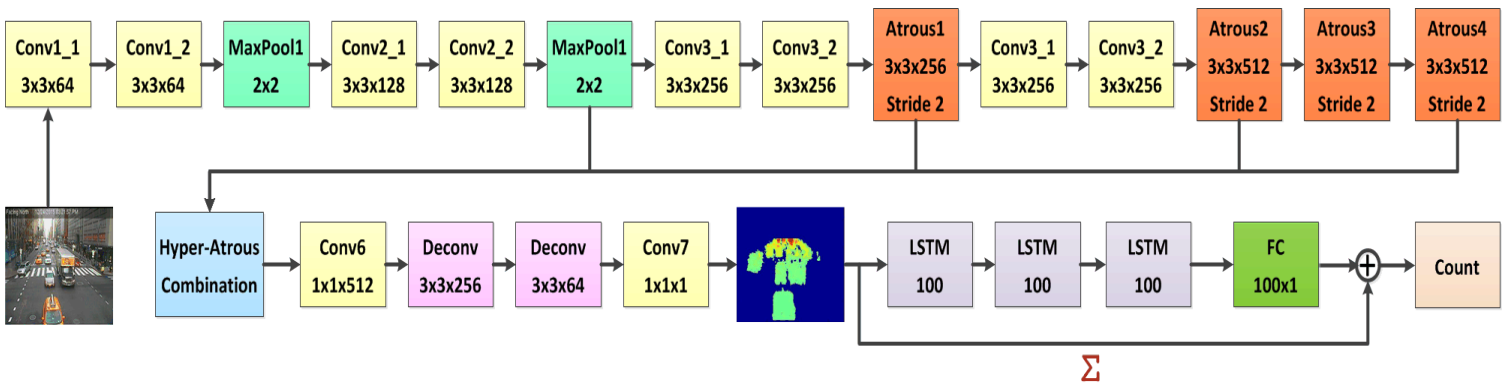
\includegraphics[width=0.9\linewidth]{ChapterThree/fcn_rlstm.png}
	\caption{Architecture of the FCN-rLSTM model (reprinted from \citet{Zhang2017}).}
	\label{fig:fcn_rlstm}
\end{figure}

\Figref{fig:fcn_rlstm} shows the full architecture of this model, from which it can be observed that the convolutional part outputs a density map $\widehat{\mD}$ which is then fed through a recurrent subnetwork responsible for producing the predicted vehicle count $\widehat{y}^{(t)}$. Training this model then implies that each input frame $\mX^{(t)}$ is annotated with the corresponding ground-truth density map $\mD^{(t)}$ and vehicle count $y^{(t)}$. The loss function is defined as:
\begin{equation}
	L(\vtheta) = \frac{1}{n} \sum_{i=1}^{n} ||\widehat{\mD}^{(t)}_i - \mD^{(t)}_i||^2_F + \frac{\lambda_c}{n} \sum_{i=1}^{n} ||\widehat{y}^{(t)}_i - y^{(t)}_i||^2,
\end{equation}
where $||\cdot||_F$ is the Frobenius norm, $\lambda_c > 0$ is a hyperparameter controlling the relative weight of the vehicle counting loss, and the dependency of $\widehat{\mD}^{(t)}_i$ and $\hat{y}^{(t)}_i$ on the network parameters $\vtheta$ is omitted to ease the notation.

\subsection{Combining MDAN and FCN-rLSTM}
We now explore several possibilities to combine MDAN and FCN-rLSTM into a single model capable of accurately counting vehicles in images from a target camera, provided that at training time we only have access to annotated data from other cameras and unlabeled data from the target.

\subsubsection{Non-temporal model}
The non-temporal model uses a sub-network in the FCN-rLSTM model as its backbone. It consists in a simplification of this, by not using LSTMs or making any other consideration on the temporal or sequential nature of the data. Figure \ref{fig:non_temporal_model} shows the architecture of the non-temporal model.

\begin{figure}[!ht]
	\centering
	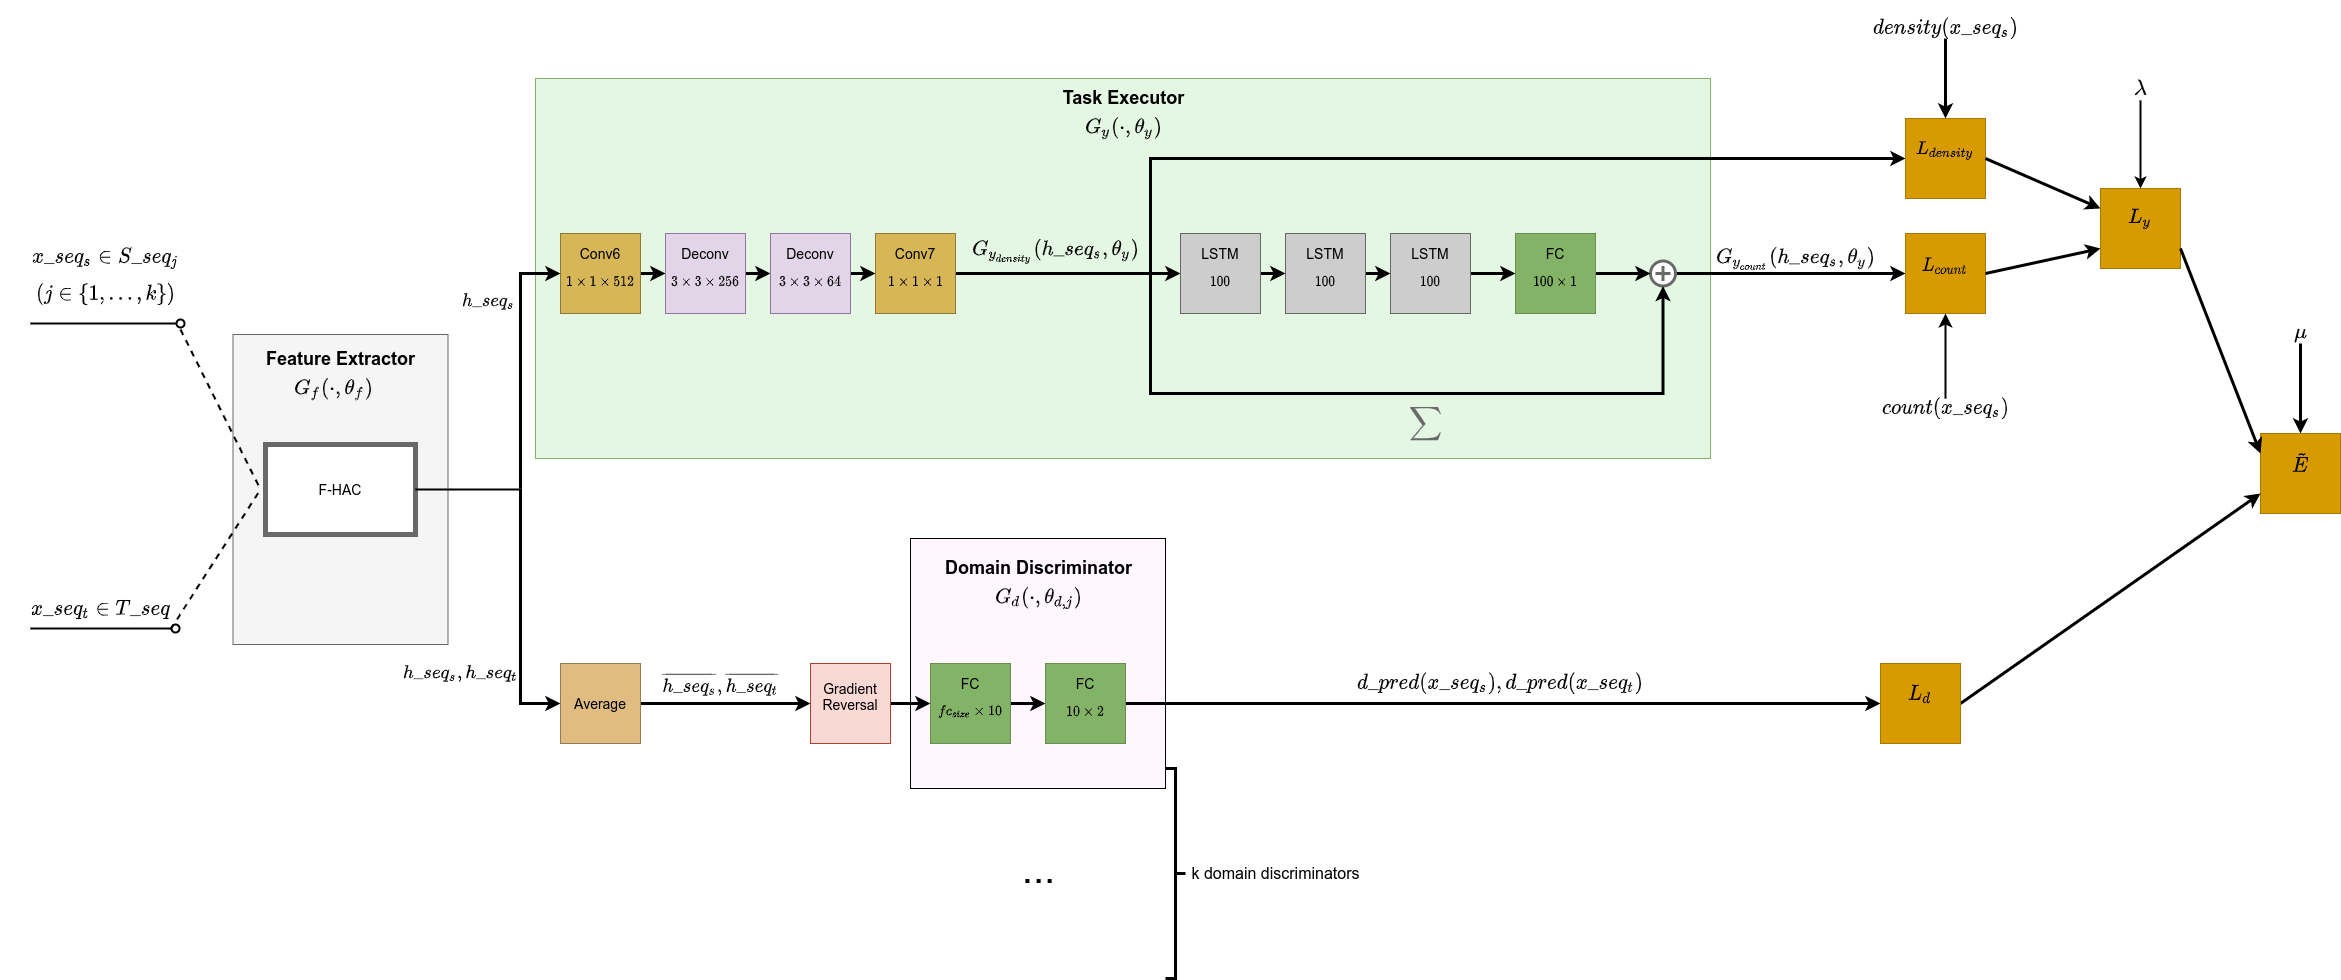
\includegraphics[width=1.0\textwidth]{ChapterThree/non_temporal.png}
	\caption{Non-temporal model. Reprinted from \citet{ThesisFrancisco}.}
	\label{fig:non_temporal_model}
\end{figure}

The component F-HAC in that figure corresponds to all layers of the FCN-rLSTM up to the hyper-atrous combination. It is used as a feature extractor, whereas the rest of the convolutional layers are used for the object counting task.

This model will be our baseline as we are primarily interested in merging the benefits of DA techniques and sequential modeling.

\subsubsection{Temporal regression model}
The temporal regression model uses the whole FCN-rLSTM model for the desired regression task, but the domain discriminator is still non-sequential, as shown in \Figref{fig:non_temporal_model}. Thus, in this model, the domain discrimination task only takes into account the domain-specific information provided by each frame individually and does not account for the domain-specific temporal dynamics that may exist.

\begin{figure}[!ht]
	\centering
	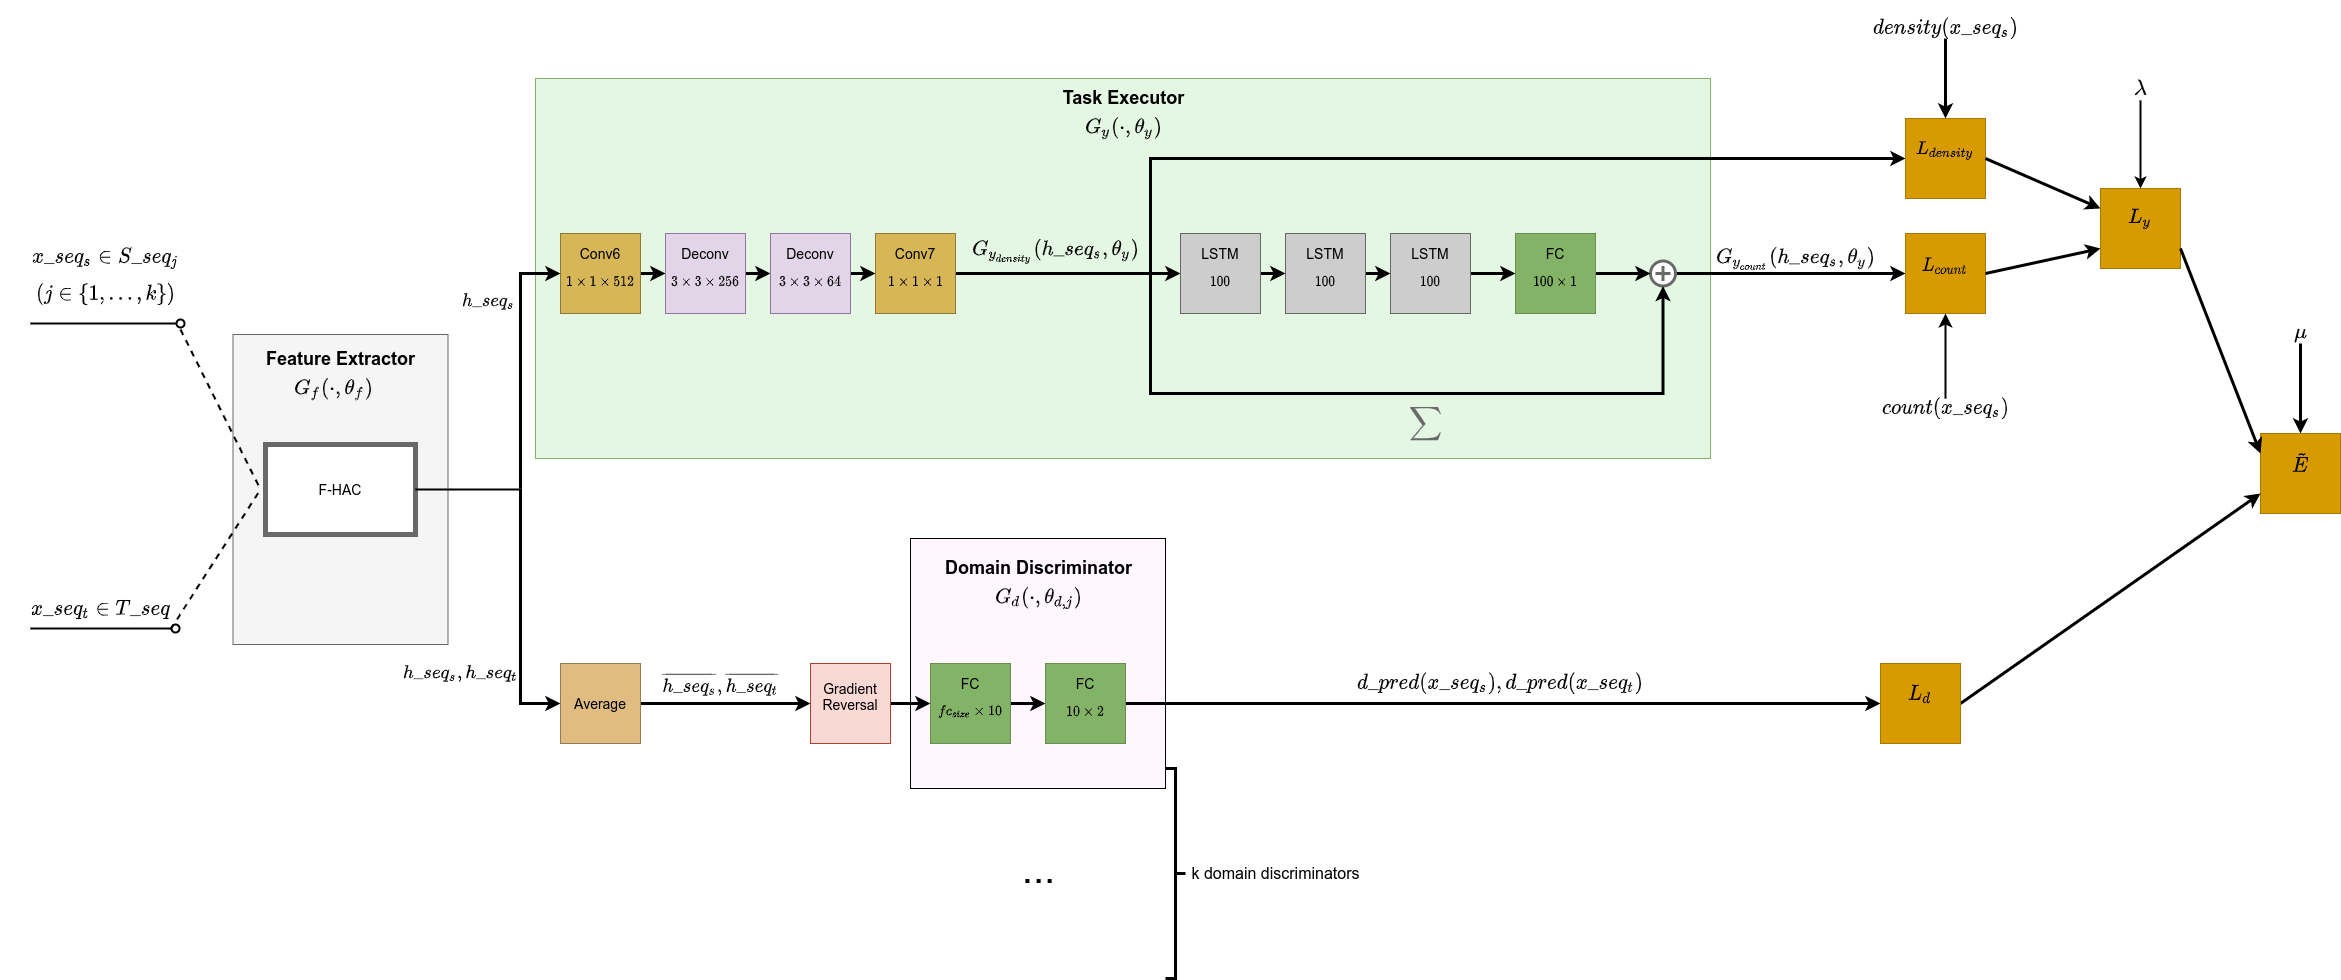
\includegraphics[width=1.0\textwidth]{ChapterThree/non_temporal.png}
	\caption{Temporal regression model. Reprinted from \citet{ThesisFrancisco}.}
	\label{fig:non_temporal_model}
\end{figure}